\documentclass[conference]{IEEEtran}
\usepackage{graphicx,booktabs,amsmath}
\usepackage[hidelinks]{hyperref}
\title{TrialMatch: Evidence-Grounded Clinical Trial Screening with Explicit Transformer Decoding}
\author{\IEEEauthorblockN{Muhammad Shaffan Ahmad}
\IEEEauthorblockA{23i-0673, Generative AI, Section A\\FAST-NUCES, Islamabad}}
\begin{document}
\maketitle
\begin{abstract}
TrialMatch predicts an expert eligibility category for each trial criterion and resolves cited sentence identifiers to source text. On 206 validation annotations, a Qwen2.5-1.5B-Instruct LoRA adapter achieved 73.79\% accuracy, 44.78\% classification macro-F1 and 62.98\% evidence micro-F1. A class-weighted variant did not recover the rare labels and reduced evidence F1. Explicit cached and speculative greedy generation matched uncached output on an NVIDIA L4. At 1024 input and 128 output tokens, caching achieved a 2.69$\times$ speedup. Speculation accelerated repetitive inputs but slowed a single screening diagnostic. Tiled attention reduced incremental allocation with a latency cost. A browser app presents decisions, source evidence, export and decoder comparison. Held-out performance remains unmeasured.
\end{abstract}
\begin{IEEEkeywords}
clinical trial screening, evidence retrieval, LoRA, KV cache, online softmax, speculative decoding
\end{IEEEkeywords}
\section{Introduction and Related Work}
TrialGPT separates retrieval, criterion matching and ranking \cite{trialgpt}. We use its expert criterion annotations \cite{dataset} for evidence-grounded matching with a locally executable model. Each criterion is evaluated against a numbered note. The browser resolves predicted sentence identifiers to exact text and applies explicit aggregation rules.

The Transformer defines scaled dot-product attention and causal masking \cite{transformer}. Qwen2.5 supplies decoder-only models for adaptation \cite{qwen}. LoRA freezes base parameters and learns low-rank updates \cite{lora}. FlashAttention motivates tiling and online softmax through lower memory traffic \cite{flash}; we implement its recurrence independently of fused kernels. Leviathan et al. use draft predictions and parallel target verification \cite{spec}; our implementation specializes the procedure to greedy decoding. Transformers supplies KV storage while project code controls the forward loop and cache positions \cite{cache}.
\section{Materials and Methods}
\subsection{Dataset and adaptation}
The fixed TrialGPT snapshot contains 1,015 annotations from 53 patients. Sorted unique patient IDs are shuffled with NumPy \texttt{default\_rng(42)}, then split 37/8/8, yielding 603/206/206 annotations. The manifest records patient IDs, counts, revision and source hash. Only note, criterion type and criterion text enter the prompt. Expert labels and evidence IDs are targets. GPT-generated fields are excluded from both.

The Apache-2.0 Qwen2.5-1.5B-Instruct target has 1.54B parameters, 28 layers, 12 query heads and two KV heads. The 0.49B draft has 24 layers, 14 query heads and two KV heads \cite{qwen,models}. Both use RoPE, grouped-query attention and a 32,768-token context. Weight-only BF16 estimates are 3.08 and 0.98 GB. The larger model provides the target capacity within the compute budget, and the smaller model reduces drafting cost. Vocabulary mapping, special IDs, chat templates and encoding probes agreed.

We used assistant-token cross-entropy with prompt and padding masked. LoRA rank was 16, scaling 32 and dropout 0.05 on attention and MLP projections. AdamW used learning rate $2\times10^{-4}$, weight decay 0.01, norm clipping 1.0, 10\% warm-up and linear decay. Three epochs used microbatch two and four accumulation steps with supervised-token normalization. All 603 v2 rows fit the 2,048-token limit (maximum 786). The historical run used a T4. The paired v2 runs used an A100 40 GB with BF16, PyTorch 2.14.1, Transformers 4.57.1 and PEFT 0.17.1.

Prompt v2 defines label polarity, unknown information and non-applicability and supplies a quoted JSON example. A uses ordinary loss. B weights training examples by $\min(3,\sqrt{n_{t,\max}/n_{t,c}})$ for class $c$ in type $t$, normalized to mean one. Both runs use the same rows and 228 updates. Selection maximizes validation macro-F1, then evidence micro-F1, then favors earlier epochs. A epoch 3 was selected. Reloading it reproduced its validation outputs.
\subsection{Explicit decoding and attention}
Uncached greedy recomputes the entire prefix. Cached greedy prefills once and feeds one new token per step. Calls specify absolute positions and a mask spanning the existing and new tokens. The model applies causal masking and stores projected keys and values. Cache size grows linearly with processed length. Floating-point differences from different matrix shapes can change a near-tied argmax, motivating token-level checks.

For each query row and score tile $S$, tiled attention maintains maximum $m$, normalizer $l$ and value accumulator $a$:
\begin{align}
m' &= \max(m,\max_j S_j),\\
l' &= e^{m-m'}l+\sum_j e^{S_j-m'},\\
a' &= e^{m-m'}a+\sum_j e^{S_j-m'}V_j.
\end{align}
The output is $a/l$. Absolute positions support rectangular causal masks. Fully masked tiles avoid differences of infinities. The dense reference materializes scores and uses stable softmax. Lower-precision inputs accumulate in FP32.

Speculation drafts up to four tokens and verifies the block in one target pass. The first candidate uses saved prefix logits. Each later candidate uses logits at the preceding position. Both caches are cropped to the accepted prefix at rejection, then receive the target correction token. Full acceptance can yield a target bonus token. EOS and length limits apply to committed tokens.
\subsection{Browser workflow}
Input $\to$ numbered note $\to$ criterion prompt $\to$ decoder $\to$ JSON validation $\to$ source evidence and export. The app preserves supplied IDs, rejects malformed results and flags explicit disqualifying categories as potential conflicts. Invalid, uncertain or uncited decisions require review. All-inapplicable assessments remain unassessed. The HTML and JSON downloads carry provenance. The comparison view rotates decoder order across three or five timed repeats. Figure~\ref{fig:app} shows the browser form. The supplied demo is \href{https://youtu.be/7SLR7LBg0mo}{youtu.be/7SLR7LBg0mo}.
\begin{figure}[t]
\centering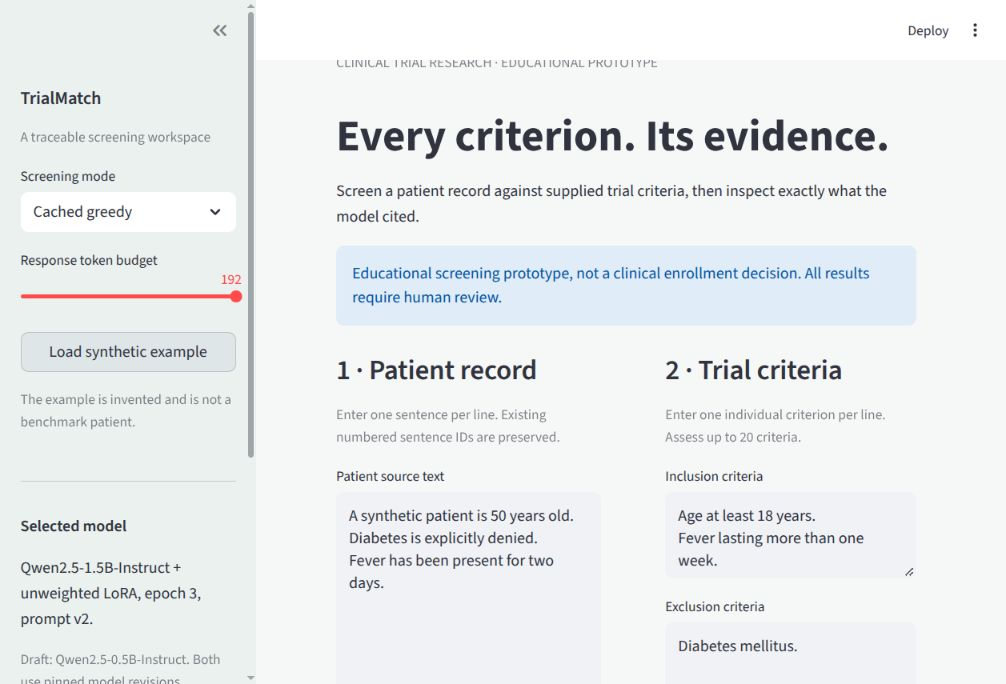
\includegraphics[width=\columnwidth]{figures/browser-preview.png}
\caption{Standalone app with synthetic input. The demo link shows the workflow.}\label{fig:app}
\end{figure}
\section{Evaluation Protocol}
Paired validation uses identical 206 annotations, batch four, greedy decoding, 192 new tokens and a strict JSON parser. Invalid responses count as incorrect. Macro-F1 averages the fixed applicable categories. Evidence micro P/R/F1 pools actual ID matches. Macro averages per example: two empty sets score one for valid outputs and one empty set scores zero. Invalid responses score zero per case and supply an empty set to micro counts. All-empty micro scores are undefined.

GPU inference used BF16 eager model attention on an L4, two warmups and five synchronized repeats. Both models stayed resident across decoder modes. Fixed-work cases disable EOS, and a separate synthetic screening case uses EOS. Ordinary prefill includes the first argmax and speculative prefill includes both models. Allocation peaks are PyTorch device measurements. Tiled attention is measured separately in FP32.
\section{Results and Discussion}
\begin{table}[t]
\centering\caption{Validation only, 206 annotations}\label{tab:validation}
\setlength{\tabcolsep}{4pt}
\begin{tabular}{lrrrr}\toprule
Recipe & Acc. & Macro F1 & Ev. micro F1 & Invalid\\\midrule
Base v1 (T4) & .0049 & .0098 & .0585 & 163\\
LoRA v1 (T4) & .7039 & .4119 & .5323 & 0\\
Base v2 (A100) & .1845 & .2059 & .1100 & 0\\
A: v2 unweighted & .7379 & .4478 & .6298 & 0\\
B: v2 weighted & .7427 & .4420 & .4751 & 0\\\bottomrule
\end{tabular}
\end{table}
Table~\ref{tab:validation} separates the historical T4 run from the controlled A100 comparison. The v2 base removes invalid JSON yet still overpredicts excluded. LoRA substantially improves its paired validation result. B gains one correct class decision but citation precision falls from .6167 to .3482 while recall rises from .6435 to .7478. B produces 161 false-positive citations versus A's 46. Both miss the rare excluded and not-included categories. Figure~\ref{fig:curve} shows the training loss and selection measurements for A.
\begin{figure}[t]
\centering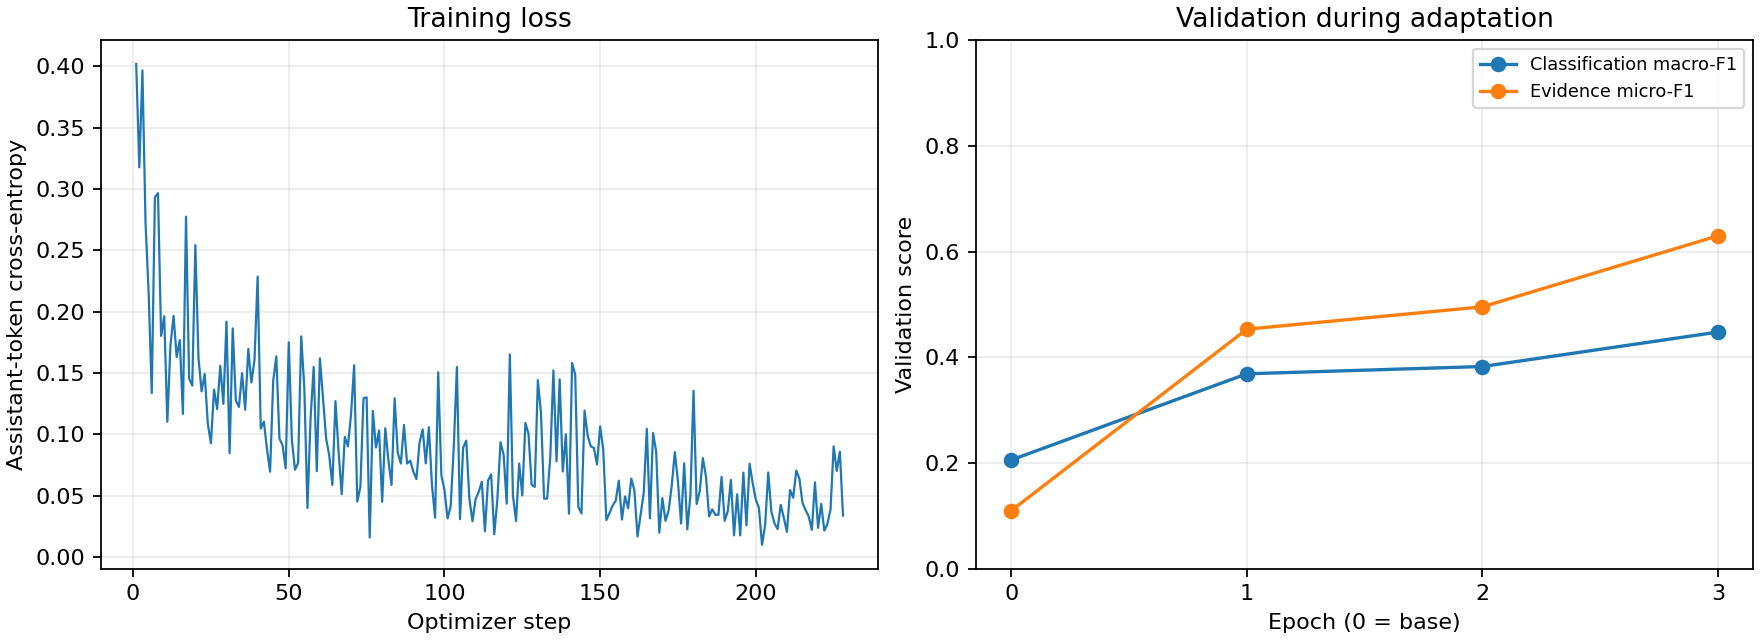
\includegraphics[width=\columnwidth]{figures/training-validation.png}
\caption{A's measured learning curves. Epoch zero denotes the untouched base.}\label{fig:curve}
\end{figure}
Table~\ref{tab:detail} breaks down the selected model by criterion type. Table~\ref{tab:classes} gives per-class precision, recall and F1. The confusion matrices in Table~\ref{tab:confusion} show that the frequent not-excluded prediction absorbs many uncertain exclusion cases.
\begin{table*}[t]
\centering\caption{Selected adapter validation by criterion type}\label{tab:detail}
\begin{tabular}{lrrrrr}
\toprule
Scope & N & Accuracy & Class macro F1 & Evidence micro P/R/F1 & Evidence macro P/R/F1\\\midrule
Overall & 206 & 0.738 & 0.448 & 0.617/0.643/0.630 & 0.799/0.807/0.794\\
Inclusion & 66 & 0.727 & 0.375 & 0.625/0.746/0.680 & 0.763/0.804/0.761\\
Exclusion & 140 & 0.743 & 0.432 & 0.600/0.500/0.545 & 0.817/0.809/0.809\\
\bottomrule
\end{tabular}
\end{table*}
\begin{table}[t]
\centering\caption{Per-class validation scores. EX/IN denote excluded/included, NA not applicable, NEI insufficient information, NEX/NIN not excluded/not included.}\label{tab:classes}
\begin{tabular}{llrrrr}
\toprule
Scope & Label & N & P & R & F1\\\midrule
Overall & EX & 2 & 0.000 & 0.000 & 0.000\\
Overall & IN & 35 & 0.862 & 0.714 & 0.781\\
Overall & NA & 12 & 0.556 & 0.417 & 0.476\\
Overall & NEI & 53 & 0.596 & 0.585 & 0.590\\
Overall & NEX & 101 & 0.784 & 0.901 & 0.839\\
Overall & NIN & 3 & 0.000 & 0.000 & 0.000\\
Inclusion & IN & 35 & 0.862 & 0.714 & 0.781\\
Inclusion & NA & 1 & 0.000 & 0.000 & 0.000\\
Inclusion & NEI & 27 & 0.622 & 0.852 & 0.719\\
Inclusion & NIN & 3 & 0.000 & 0.000 & 0.000\\
Exclusion & EX & 2 & 0.000 & 0.000 & 0.000\\
Exclusion & NA & 11 & 0.556 & 0.455 & 0.500\\
Exclusion & NEI & 26 & 0.533 & 0.308 & 0.390\\
Exclusion & NEX & 101 & 0.784 & 0.901 & 0.839\\
\bottomrule
\end{tabular}
\end{table}
\begin{table}[t]
\centering\caption{Validation confusion matrices. Rows are expert labels, columns are predictions. INV is invalid. A dash indicates an inapplicable label.}\label{tab:confusion}
\setlength{\tabcolsep}{4pt}
\begin{tabular}{llrrrrrrr}
\toprule
Scope & Gold & EX & IN & NA & NEI & NEX & NIN & INV\\\midrule
Overall & EX & 0 & 0 & 0 & 0 & 2 & 0 & 0\\
Overall & IN & 0 & 25 & 0 & 10 & 0 & 0 & 0\\
Overall & NA & 0 & 0 & 5 & 1 & 6 & 0 & 0\\
Overall & NEI & 0 & 4 & 1 & 31 & 17 & 0 & 0\\
Overall & NEX & 0 & 0 & 3 & 7 & 91 & 0 & 0\\
Overall & NIN & 0 & 0 & 0 & 3 & 0 & 0 & 0\\
Inclusion & IN & -- & 25 & 0 & 10 & -- & 0 & 0\\
Inclusion & NA & -- & 0 & 0 & 1 & -- & 0 & 0\\
Inclusion & NEI & -- & 4 & 0 & 23 & -- & 0 & 0\\
Inclusion & NIN & -- & 0 & 0 & 3 & -- & 0 & 0\\
Exclusion & EX & 0 & -- & 0 & 0 & 2 & -- & 0\\
Exclusion & NA & 0 & -- & 5 & 0 & 6 & -- & 0\\
Exclusion & NEI & 0 & -- & 1 & 8 & 17 & -- & 0\\
Exclusion & NEX & 0 & -- & 3 & 7 & 91 & -- & 0\\
\bottomrule
\end{tabular}
\end{table}


All 45 timed runs matched uncached tokens. Table~\ref{tab:decoding} reports elapsed medians. At 1024/128, cached and speculative peaks were 4.20 and 4.51 GiB allocated. Prefill/decode were 0.205/27.101 s uncached, 0.187/9.951 s cached and 0.259/8.509 s speculative. The repetitive input yielded 100\% draft acceptance. The EOS-aware screening diagnostic also matched, but accepted 12/18 candidates and took 1.62 s versus 1.27 s cached, about 28\% longer. The latter is a single diagnostic.
\begin{table}[t]
\centering\caption{L4 decoding, median seconds}\label{tab:decoding}
\setlength{\tabcolsep}{4pt}
\begin{tabular}{lrrrr}\toprule
In/out & Uncached & Cached & Spec. & Spec. tok/s\\\midrule
128/32 & 2.603 & 2.535 & 2.268 & 14.11\\
512/64 & 5.722 & 5.000 & 4.334 & 14.77\\
1024/128 & 27.306 & 10.147 & 8.769 & 14.60\\\bottomrule
\end{tabular}
\end{table}
Tiled attention matched dense across causal, noncausal and rectangular cases. Maximum absolute error was $5.96\times10^{-7}$ and largest mean error was $3.07\times10^{-8}$. At length 1024 incremental allocation peaked at 33.02 MiB dense and 1.19 MiB tiled. Median times were 1.263 and 305.160 ms, respectively. Many small PyTorch operations add launch overhead in the standalone educational implementation.
\subsection{Eight validation errors}
Annotation IDs identify the saved prediction records.
\begin{enumerate}
\item \textbf{31, fever duration.} The model cites two days and predicts insufficient information for more than one week. The expert marks not included. Relevant evidence was found but the comparison failed.
\item \textbf{41, respiratory distress.} Sentence 4 documents distress. The model cites it but predicts not excluded, reversing the expert exclusion decision.
\item \textbf{8, unstable angina.} The model cites three symptom sentences and predicts not excluded. The expert label is insufficient information. Related symptoms leave the condition unresolved.
\item \textbf{21, hypertension.} The model cites documented hypertension yet returns insufficient information. The expert marks included. Retrieval and classification disagree.
\item \textbf{24, PCI/CABG context.} It predicts not excluded without evidence where the expert marks not applicable. It confuses absence of a condition with irrelevance.
\item \textbf{33, inconclusive workup.} It predicts insufficient information where the expert marks not applicable. Both evidence sets are empty, showing why evidence agreement can coexist with a class error.
\item \textbf{235, fibroid-associated symptoms.} The model infers included, cites related findings and omits expert sentence 5. The expert finds insufficient information for the attribution.
\item \textbf{241, uterine level.} The model cites ultrasound dimensions in sentence 4 and predicts insufficient information. The expert cites exam sentence 1 and marks not excluded. Both source selection and classification differ.
\end{enumerate}
\section{Limitations and Conclusion}
The small eight-patient validation group, sparse labels, checkpoint selection, and synthetic timing inputs limit generalization. The held-out comparison is pending. The included frozen evaluation script measures base and adapter on the prescribed test split using identical prompts and settings. TrialMatch is an educational prototype requiring human enrollment review.
\appendices
\section{Reproduction and AI Use}
Source repository supplied by the author: \href{https://github.com/M-Shaffan-Ahmad/TrialMatch-A-traceable-screening-workspace}{TrialMatch on GitHub}. The source archive includes the pinned model and split manifests, measured logs and the training, benchmark and app workflows. Notebook 06 runs frozen test evaluation. The supplied adapter ZIP carries the selected weights and tokenizer. An external adapter download URL remains to be supplied.

OpenAI Codex assisted with implementation, testing, notebooks, experiment review and report preparation. Transformers and PEFT supply model and adapter support. PyTorch supplies tensor operations, and Streamlit supplies the UI. Custom project code implements the decoding loops, speculative cache control and tiled recurrence. Reported results derive from exported measurements.
\bibliographystyle{IEEEtran}
\bibliography{references}
\end{document}
